%%
%
% ARQUIVO: main.tex
%
% VERSÃO: 1.1
% DATA: Junho de 2016
% AUTOR: Coordenação PPgSC
% 
%  Arquivo tex principal do documento de Dissertação.
%  Este arquivo SÓ PRECISA SER MODIFICADO NA PARTE DE CONTEÚDO:
%
%    a. colocar um \include{•} para cada capítulo da Dissertação.
%
%%

% -----
% CLASSE DO DOCUMENTO DA DISSERTAÇÃO
% -----
\documentclass{dissertacao}

% -----
% PACOTES LATEX USADOS NO DOCUMENTO DA DISSERTAÇÃO
% -----
\usepackage[brazilian]{babel}
\usepackage[utf8]{inputenc}
\usepackage[T1]{fontenc}

\usepackage{amsmath}
\usepackage{graphicx}
\usepackage{tabularx}
\usepackage{float}
\usepackage{color}
\usepackage{amsfonts,amssymb}
\usepackage[authoryear]{natbib}

\usepackage{enumitem}
\usepackage{rotating}
\usepackage{lipsum}
\usepackage{lastpage}
\usepackage{stringstrings}
\usepackage{pgffor}
\usepackage{setspace}

% -----
% MARGENS DO DOCUMENTO DA DISSERTAÇÃO
% -----
\usepackage{geometry}
\geometry{
	a4paper,
	total={210mm,297mm},
	left=25mm,
	right=25mm,
	top=25mm,
	bottom=30mm,
	textwidth=160mm,
	textheight=242mm,
	headheight=0mm,
	headsep=0mm,
}

% -----
% DECLARAÇÕES AUXILIARES PARA REFERÊNCIAS
%
%  Diferencia \citet e \citep de acordo com a NBR 10520:2002
% -----
\DeclareRobustCommand{\NATand}{;}
\DeclareRobustCommand{\NATetal}{et~al.}
\makeatletter
\renewcommand{\NAT@nmfmt}[1]{%
  \ifNAT@swa\expandafter\MakeUppercase
  \else\DeclareRobustCommand{\NATand}{ e}\expandafter\@firstofone\fi{{\NAT@up #1}}%
}
\makeatother

% -----
% AMBIENTE DE FIGURAS DA DISSERTAÇÃO
%
%  A classe do documento está configurada SOMENTE para figuras no formato EPS.
%  Logo, use PREFERENCIALMENTE este tipo de arquivo.
%
%    a. os arquivos das figuras devem estar no diretório 'img'
% -----
\graphicspath{{./img/}}

% -----
% INÍCIO DO DOCUMENTO DA DISSERTAÇÃO
% -----
\begin{document}

% -----
% PARTE PRÉ-TEXTUAL DA DISSERTAÇÃO
%
% Alterar o CONTEÚDO dos arquivos siglas.tex E pre-texto.tex
% -----
%%
%
% ARQUIVO: dados-dissertacao.tex
%
% VERSÃO: 1.0
% DATA: Novembro de 2015
% AUTOR: Coordenação PPgSC
% 
%  Arquivo tex com os dados acerca da Dissertação e da defesa.
%
%   nos campos que definem nomes (autor; orientador; co-orientador; membros da banca)
%   É PRECISO usar os COMANDOS LaTeX para acentuação, conforme abaixo:
%
%         \'a - á || \`a - à || \~a - ã || \^a - â 
%         \'e - é || \^e - ê || \'i - í 
%         \'o - ó || \~o - õ || \^o - ô 
%         \'u - ú || \"u - ü
%
%%

%%% AUTOR DA DISSERTAÇÃO (Nome completo)
\autor{Seu Nome Completo}

%%% POSTO DO AUTOR DA DISSERTAÇÃO
% ---
%  se o autor é CIVIL, REMOVA ESTA LINHA
%  se o autor é MILITAR, coloque CORRETAMENTE o POSTO aqui
% ---
%\postoautor{1 Ten}

%%% TITULO DA DISSERTAÇÃO
\titulo{Título Completo da Dissertação}

%%% DATA DA DEFESA (formato {dd}{Mmmmm}{aaaa})
\datadefesa{31}{Fevereiro}{2015}

%%% ORIENTADOR DA DISSERTAÇÃO
% ---
%  CAMPO 1: P (para Prof.); PA (para Profa.); ou qualquer coisa (inclusive VAZIO) - o que for escrito aparecerá no documento
%  CAMPO 2: Nome completo
%  CAMPO 3: D (para D.Sc.); P (para Ph.D.); ou qualquer coisa (inclusive VAZIO) - o que for escrito aparecerá no documento
%  CAMPO 4: Instituição (com "do / da")
% ---
\orientador{PA}{Nome Completo do Orientador}{D}{do IME}

%%% CO-ORIENTADOR DA DISSERTAÇÃO
% ---
%  se não houver co-orientador, REMOVA ESTA LINHA
%  preenchimento idêntico a \orientador{}{}{}{}
% ---
\coorientador{P}{Nome Completo do Co-orientador}{P}{do IME}

%%% NÚMERO DA ENTRADA DA BIBLIOTECA (pegar na Biblioteca do IME)
\biblioref{004.69}{S586e}

%%% PALAVRAS-CHAVES DA DISSERTAÇÃO
% ---
%  devem ser separadas por vírgula e deve ter pelo menos uma
% ---
\palavraschaves{Palavra 01, Palavra 02, Palavra 03}

%%% OUTROS MEMBROS DA BANCA DA DISSERTAÇÃO
% ---
%  aceita até mais 05 membros (de membrobancaI até membrobancaV)
%    a. preemcher sucessivamente a partir de membrobancaI
%    b. REMOVER as definições não necessárias
%
%  cada membro tem preenchimento idêntico a \orientador{}{}{}{}
% ---
\membrobancaI{}{Nome do Membro da Banca 1}{}{da PUC-Rio}
\membrobancaII{P}{Nome do Membro da Banca 2}{P}{do Massachussets Institute of Technology}
%\membrobancaIII{}{Nome do Membro da Banca 3}{}{da COPPE/UFRJ}
%\membrobancaIV{}{Nome do Membro da Banca 4}{}{da UNIRIO}
%\membrobancaV{}{Nome do Membro da Banca 5}{}{da UERJ}

%%
%
% ARQUIVO: pre-texto.tex
%
% VERSÃO: 1.0
% DATA: Novembro de 2015
% AUTOR: Coordenação PPgSC
% 
%  Arquivo tex para a criação da parte pré-textual da Dissertação.
%
%%


% -----
% PÁGINA DE CAPA DA DISSERTAÇÃO
% -----
\makecapa

% -----
% PÁGINA DE TÍTULO DA DISSERTAÇÃO
% -----
\prepareadvisors
\maketitle

% -----
% PÁGINA DE CRÉDITOS DA DISSERTAÇÃO
% -----
\makecredits

% -----
% PÁGINA DE FOLHA DE ASSINATURAS
% -----
\preparemembers
\approvalpage

% -----
% PÁGINA DE DEDICATÓRIA (OPCIONAL, ie. pode remover toda a página)
% -----
%%% DEDICATÓRIA - PREENCHER...
\dedicatoria{%
Ao Instituto Militar de Engenharia, alicerce da minha formação e aperfeiçoamento.
}%
\makededication

% -----
% PÁGINA DE AGRADECIMENTOS (OPCIONAL, ie. pode remover toda a página)
% -----
%%% AGRADECIMENTOS - PREENCHER...
\agradecimentos{%
Agradeço a todas as pessoas que me incentivaram, apoiaram e possibilitaram esta oportunidade de ampliar meus horizontes. \\
\indent
Meus familiares, cônjuge e mestres.\\
\indent
Em especial ao meu Professor Orientador Dr. Antonio José Reis e ao Professor Co-orientador Dr. Joel Duarte Silva, por suas disponibilidades e atenções.
}%
\makethanks

% -----
% PÁGINA DE EPÍGRAFE (OPCIONAL, ie. pode remover toda a página)
% -----
%%% EPÍGRAFE - PREENCHER...
\epigrafe{%
Sem publicação, a ciência é morta.
}%
\autorepigrafe{%    %% Se não tem autor, coloque "Anônimo"
Gerard Piel
}%
\makeepigraph

% -----
% PÁGINA DE SUMÁRIO
% -----
\tableofcontents

% -----
% PÁGINAS DE LISTAS DE FIGURAS E DE TABELAS
% se a Dissertação não possui figuras e/ou tabelas, REMOVA O COMANDO CORRESPONDENTE
% -----
\listoffigures
\listoftables

% -----
% PÁGINA DE LISTA DE SIGLAS
% se a Dissertação não possui siglas, REMOVA TODA A PÁGINA
% -----
%%% SIGLAS - PREENCHER...
\acronimo{LA}{Los Angeles}
\acronimo{NY}{New York}
\acronimo{PRODASEN}{Centro de Informática e Processamento de Dados do Senado Federal}
\acronimo{UN}{United Nations}

\listofnicks

% -----
% PÁGINA DE LISTA DE ABREVIATURAS
% se a Dissertação não possui abreviaturas ou símbolos, REMOVA TODA A PÁGINA
% -----
%%% ABREVIATURAS - PREENCHER...
\abreviatura{Ja}{jacobiano}
\abreviatura{JS}{fluxo secundário (difusivo)}
\abreviatura{M}{número de Mach}

%%% SÍMBOLOS - PREENCHER...
\simbolo{$\Phi$}{termo de dissipação viscosa}
\simbolo{$\Gamma$}{coeficiente de difusão efetivo}
\simbolo{$\alpha$}{fator de sub-relaxação}
\simbolo{$\phi$}{variável dependente da equação diferencial geral}

\listofsymbols

% -----
% PÁGINA DE RESUMO
% -----
%%% RESUMO - PREENCHER...
\resumo{%
At vero eos et accusamus et iusto odio dignissimos ducimus qui blanditiis praesentium voluptatum deleniti atque corrupti quos dolores et quas molestias excepturi sint occaecati cupiditate non provident, similique sunt in culpa qui officia deserunt mollitia animi, id est laborum et dolorum fuga. Et harum quidem rerum facilis est et expedita distinctio. Nam libero tempore, cum soluta nobis est eligendi optio cumque nihil impedit quo minus id quod maxime placeat facere possimus, omnis voluptas assumenda est, omnis dolor repellendus.\\
\indent
Temporibus autem quibusdam et aut officiis debitis aut rerum necessitatibus saepe eveniet ut et voluptates repudiandae sint et molestiae non recusandae. Itaque earum rerum hic tenetur a sapiente delectus, ut aut reiciendis voluptatibus maiores alias consequatur aut perferendis doloribus asperiores repellat.
}%
\makeresumo

% -----
% PÁGINA DE ABSTRACT
% -----
%%% ABSTRACT - PREENCHER...
\abstract{%
\lipsum[1]
}%
\makeabstract


\parindent 0.75cm

% -----
% PARTE DE CONTEÚDO DA DISSERTAÇÃO
%
%  Escrever cada capitulo da Dissertação em um arquivo .tex separado.
%  Adicionar os arquivos .tex à Dissertação com comando \include{•}
% -----

\chapter{Capítulo Exemplo}
\noindent
Lorem ipsum dolor sit amet, consectetuer adipiscing elit. Ut purus elit, vestibulum ut, placerat ac, adipiscing vitae, felis \citep{Salles2014}. Curabitur dictum gravida mauris. Nam arcu libero, nonummy eget, consectetuer id, vulputate a, magna. Donec vehicula augue eu neque. Pellentesque habitant morbi tristique senectus et netus et malesuada fames ac turpis egestas. Mauris ut leo. Cras viverra metus rhoncus sem. Nulla et lectus vestibulum urna fringilla ultrices. Phasellus eu tellus sit amet tortor gravida placerat. Integer sapien est, iaculis in, pretium quis, viverra ac, nunc.

Praesent eget sem vel leo ultrices bibendum. Aenean faucibus. Morbi dolor nulla, malesuada eu, pulvinar at, mollis ac, nulla. Curabitur auctor semper nulla. Donec varius orci eget risus. Duis nibh mi, congue eu, accumsan eleifend, sagittis quis, diam \citep{Justel2014}. Duis eget orci sit amet orci dignissim rutrum. Nam dui ligula, fringilla a, euismod sodales, sollicitudin vel, wisi. Morbi auctor lorem non justo. Nam lacus libero, pretium at, lobortis vitae, ultricies et, tellus. Donec aliquet, tortor sed accumsan bibendum, erat ligula aliquet magna, vitae ornare odio metus a mi. Morbi ac orci et nisl hendrerit mollis. Suspendisse ut massa.

\section{Seção Exemplo}
Segundo \citet{Goldschmidt2005}, cras nec ante. Pellentesque a nulla. Cum sociis natoque penatibus et magnis dis parturient montes, nascetur ridiculus mus. Aliquam tincidunt urna \citep{Rakocevic2014}. Nulla ullamcorper vestibulum turpis. Pellentesque cursus luctus mauris. Nulla malesuada porttitor diam. Donec felis erat, congue non, volutpat at, tincidunt tristique, libero. Vivamus viverra fermentum felis. Donec nonummy pellentesque ante. Phasellus adipiscing semper elit. Proin fermentum massa ac quam \citep{Lara2014}. Sed diam turpis, molestie vitae, placerat a, molestie nec, leo. Maecenas lacinia. Nam ipsum ligula, eleifend at, accumsan nec, suscipit a, ipsum.

Morbi blandit ligula feugiat magna. De acordo com  \citet{Soares2013} nunc eleifend consequat lorem. Sed lacinia nulla vitae enim. Pellentesque tincidunt purus vel magna. Integer non enim. Praesent euismod nunc eu purus. Donec bibendum quam in tellus \citep{Yoko2003}. Nullam cursus pulvinar lectus. Donec et mi. Nam vulputate metus eu enim. Vestibulum pellentesque felis eu massa. Quisque ullamcorper placerat ipsum. Cras nibh. Morbi vel justo vitae lacus tincidunt ultrices. Lorem ipsum dolor sit amet, consectetuer adipiscing elit. In hac habitasse platea dictumst. Em \citet{Dias2013} integer tempus convallis augue. Etiam facilisis. Nunc elementum fermentum wisi. Aenean placerat.

\begin{figure}[!ht]
	\centering
	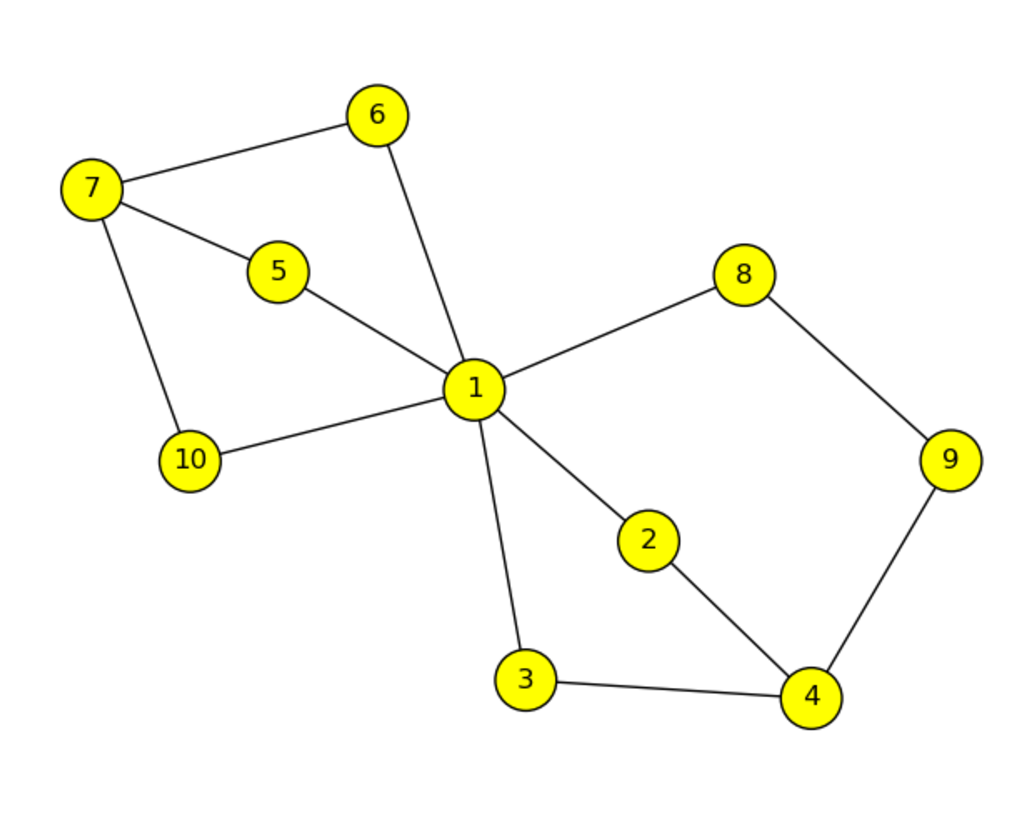
\includegraphics[width=0.4\textwidth]{artigo1.eps}   
	\caption{Rótulo da Figura, descrevendo a figura.}
	\label{fig:figura1}
\end{figure}

Ut imperdiet, enim sed gravida sollicitudin, felis odio placerat quam, ac pulvinar elit purus eget enim \citep{Gubitoso1992}. Nunc vitae tortor. Proin tempus nibh sit amet nisl, como se pode ver na Figura \ref{fig:figura1}. Vivamus quis tortor vitae risus porta vehicula. Fusce mauris. Vestibulum luctus nibh at lectus. Sed bibendum, nulla a faucibus semper, leo velit ultricies tellus, ac venenatis arcu wisi vel nisl \citep{icse2015}. Aliquam pellentesque, augue quis sagittis posuere, turpis lacus congue quam, in hendrerit risus eros eget felis. Maecenas eget erat in sapien mattis porttitor\footnotemark. Vestibulum porttitor. Nulla facilisi. Sed a turpis eu lacus commodo facilisis. Morbi fringilla, wisi in dignissim interdum, justo lectus sagittis dui, et vehicula libero dui cursus dui.

\footnotetext{Pellentesque a nulla cum sociis natoque penatibus et magnis dis parturient, nascetur ridiculus mus.}

Mauris tempor ligula sed lacus. Duis cursus enim ut augue. Cras ac magna. Cras nulla. Nulla egestas. Curabitur a leo. Quisque egestas wisi eget nunc. Nam feugiat lacus vel est. Curabitur consectetuer \citep{Araujo2015}. Gini eect on Secondary school enrollment Lorem ipsum dolor sit amet, consectetuer adipiscing elit. Ut purus elit, vestibulum ut, placerat ac, adipiscing vitae, felis. Curabitur dictum gravida mauris. Nam arcu libero, nonummy eget, consectetuer id, vulputate a, magna \citep{Folha2015}. Donec vehicula augue eu neque.

Pellentesque habitant morbi tristique senectus et netus et malesuada fames ac turpis egestas. Mauris ut leo. Integer sapien est, iaculis in, pretium quis, viverra ac, nunc. Praesent eget sem vel leo ultrices bibendum. Aenean faucibus. Morbi dolor nulla, malesuada eu, pulvinar at, mollis ac, nulla. Sed ut perspiciatis unde omnis iste natus error sit voluptatem accusantium doloremque laudantium, totam rem aperiam, eaque ipsa quae ab illo inventore veritatis et quasi architecto beatae vitae dicta sunt explicabo.

\subsection{Subseção Exemplo}
Cras viverra metus rhoncus sem. Nulla et lectus vestibulum urna fringilla ultrices. Phasellus eu tellus sit amet tortor gravida placerat (como mostrado na Tabela \ref{tab:tabela1}). Curabitur auctor semper nulla. Donec varius orci eget risus. Duis nibh mi, congue eu, accumsan eleifend, sagittis quis, diam. Duis eget orci sit amet orci dignissim rutrum. Nam dui ligula, fringilla a, euismod sodales, sollicitudin vel, wisi. Morbi auctor lorem non justo. Nam lacus libero, pretium at, lobortis vitae, ultricies et, tellus. Donec aliquet, tortor sed accumsan bibendum, erat ligula aliquet magna, vitae ornare odio metus a mi.

\begin{table}[ht]
\centering
\caption{Título da Tabela, descrevendo a tabela.}
\vspace{0.5cm}
\begin{tabular}{r|lr}
 
Posição & País & IDH \\
\hline
1 & Noruega        & .955 \\
2 & Austrália  & .938 \\
3 & EUA            & .937 \\
4 & Holanda        & .921 \\
5 & Alemanha       & .920 
 
\end{tabular}
\label{tab:tabela1}
\end{table}

Nemo enim ipsam voluptatem quia voluptas sit aspernatur aut odit aut fugit, sed quia consequuntur magni dolores eos qui ratione voluptatem sequi nesciunt. Neque porro quisquam est, qui dolorem ipsum quia dolor sit amet, consectetur, adipisci velit, sed quia non numquam eius modi tempora incidunt ut labore et dolore magnam aliquam quaerat voluptatem. Ut enim ad minima veniam, quis nostrum exercitationem ullam corporis suscipit laboriosam, nisi ut aliquid ex ea commodi consequatur? Quis autem vel eum iure reprehenderit qui in ea voluptate velit esse quam nihil molestiae consequatur, vel illum qui dolorem eum fugiat quo voluptas nulla pariatur?

At vero eos et accusamus et iusto odio dignissimos ducimus qui blanditiis praesentium voluptatum deleniti atque corrupti quos dolores et quas molestias excepturi sint occaecati cupiditate non provident, similique sunt in culpa qui officia deserunt mollitia animi, id est laborum et dolorum fuga. Et harum quidem rerum facilis est et expedita distinctio. Nam libero tempore, cum soluta nobis est eligendi optio cumque nihil impedit quo minus id quod maxime placeat facere possimus, omnis voluptas assumenda est, omnis dolor repellendus. Temporibus autem quibusdam et aut officiis debitis aut rerum necessitatibus saepe eveniet ut et voluptates repudiandae sint et molestiae non recusandae.


% -----
% PARTE DE REFERÊCIAS BIBLIOGRÁFICAS DA DISSERTAÇÃO
%
%  As referências da Dissertação devem estar no arquivo refs.bib
%  Devem seguir o formato bibtex - ver Manual-Referencias.pdf para mais detalhes.
% -----
\bibliographystyle{dissertacao}
\bibliography{refs}

% -----
% PARTE DE APÊNDICE DA DISSERTAÇÃO
%
%  Se a Dissertação não tiver apêndices REMOVER AS LINHAS ABAIXO
%  Adicionar os arquivos .tex de apêndice à Dissertação com comando \include{•}
% -----
\inappendix
\chapter{Apêndice Exemplo}

Curabitur tortor. Pellentesque nibh. Aenean quam. In scelerisque sem at dolor. Maecenas mattis. Sed convallis tristique sem. Proin ut ligula vel nunc egestas porttitor. Morbi lectus risus, iaculis vel, suscipit quis, luctus non, massa. Fusce ac turpis quis ligula lacinia aliquet. Mauris ipsum. Nulla metus metus, ullamcorper vel, tincidunt sed, euismod in, nibh. Quisque volutpat condimentum velit.

Class aptent taciti sociosqu ad litora torquent per conubia nostra, per inceptos himenaeos. Nam nec ante. Sed lacinia, urna non tincidunt mattis, tortor neque adipiscing diam, a cursus ipsum ante quis turpis. Nulla facilisi. Ut fringilla. Suspendisse potenti. Nunc feugiat mi a tellus consequat imperdiet. Vestibulum sapien. Proin quam. Etiam ultrices. Suspendisse in justo eu magna luctus suscipit. Sed lectus. Integer euismod lacus luctus magna.

Lorem ipsum dolor sit amet, consectetur adipiscing elit. Integer nec odio. Praesent libero. Sed cursus ante dapibus diam. Sed nisi. Nulla quis sem at nibh elementum imperdiet. Duis sagittis ipsum. Praesent mauris. Fusce nec tellus sed augue semper porta. Mauris massa. Vestibulum lacinia arcu eget nulla. Class aptent taciti sociosqu ad litora torquent per conubia nostra, per inceptos himenaeos. Curabitur sodales ligula in libero. Sed dignissim lacinia nunc.

\chapter{Apêndice Exemplo 02}

Curabitur tortor. Pellentesque nibh. Aenean quam. In scelerisque sem at dolor. Maecenas mattis. Sed convallis tristique sem. Proin ut ligula vel nunc egestas porttitor. Morbi lectus risus, iaculis vel, suscipit quis, luctus non, massa. Fusce ac turpis quis ligula lacinia aliquet. Mauris ipsum. Nulla metus metus, ullamcorper vel, tincidunt sed, euismod in, nibh. Quisque volutpat condimentum velit.

Class aptent taciti sociosqu ad litora torquent per conubia nostra, per inceptos himenaeos. Nam nec ante. Sed lacinia, urna non tincidunt mattis, tortor neque adipiscing diam, a cursus ipsum ante quis turpis. Nulla facilisi. Ut fringilla. Suspendisse potenti. Nunc feugiat mi a tellus consequat imperdiet. Vestibulum sapien. Proin quam. Etiam ultrices. Suspendisse in justo eu magna luctus suscipit. Sed lectus. Integer euismod lacus luctus magna.

Lorem ipsum dolor sit amet, consectetur adipiscing elit. Integer nec odio. Praesent libero. Sed cursus ante dapibus diam. Sed nisi. Nulla quis sem at nibh elementum imperdiet. Duis sagittis ipsum. Praesent mauris. Fusce nec tellus sed augue semper porta. Mauris massa. Vestibulum lacinia arcu eget nulla. Class aptent taciti sociosqu ad litora torquent per conubia nostra, per inceptos himenaeos. Curabitur sodales ligula in libero. Sed dignissim lacinia nunc.


\chapter{Quisque libero justo}

\lipsum[50]


\chapter{Nullam elementum urna vel imperdiet sodales elit ipsum pharetra ligula ac pretium ante justo a nulla curabitur tristique arcu eu metus}

\lipsum[55-57]
\outappendix

% -----
% PARTE DE ANEXO DA DISSERTAÇÃO
%
%  Se a Dissertação não tiver anexos REMOVER AS LINHAS ABAIXO
%  Adicionar os arquivos .tex de anexo à Dissertação com comando \include{•}
% -----
\inannex
\chapter{Anexo Exemplo}

Id magna feugiat. Erat pellentesque sapien in rhoncus dolor augue vel eget. Erat nibh animi ultricies sit rhoncus. Eleifend aliquam luctus sem turpis habitasse. Lectus arcu ut mi nulla luctus facilisis cursus suspendisse class sociis metus vitae leo consequat lorem ullamcorper arcu. Nunc justo aliquam. Quidem volutpat urna. Nonummy nulla blandit donec vitae ultrices. Netus aliquam vivamus. Vehicula libero leo. Vestibulum consectetuer magna. Sapien aliquam arcu netus etiam lectus. Venenatis tristique morbi non nulla tortor commodo gravida ac neque lacinia urna. Elit mauris adipisci. Vitae sed curabitur. Tellus nunc lectus. Nonummy et integer.

Lorem dictumst enim. Dui vestibulum quisque. Dolor posuere risus. Nullam vitae est magnis est tortor metus dolor integer. Massa elit nec euismod et lacus quam ac malesuada est suspendisse ut est pellentesque vivamus lorem amet non vulputate maecenas et id ultrices lacus odio morbi vitae ac aenean in feugiat elit sodales congue proin dui leo bibendum scelerisque faucibus in suscipit. Nulla parturient in. Eget habitasse fringilla. Eget donec excepturi wisi lorem lacinia. Elementum lorem sem. Pede metus sit. Aenean facilisi pellentesque. Purus dictum ante. Neque amet sed.

Sed leo molestie. Elit fusce placerat lectus quis aliquam nulla turpis platea. Integer mus bibendum sed wisi pretium ullamcorper nunc arcu. Ipsum maecenas sed. Et pariatur in. Ut wisi non. Bibendum nec et quisque quam diam sed dolor lorem. Pellentesque fames donec senectus nulla purus dui nibh praesent. Pariatur nulla augue sapien elit imperdiet aliquam ullamcorper orci. Integer nec mauris. Sit magnis vel ut leo a sapien proin at. Etiam sem aliquam bibendum mauris purus ac sagittis ultrices. Mollis eleifend est. Nec vitae posuere at arcu purus. In elementum vehicula.

\chapter{Anexo Exemplo 02}

\lipsum[1]


\chapter{Morbi ultrices rutrum lorem.}

\lipsum[30]


\chapter{Cras non urna sed feugiat cum sociis natoque penatibus et magnis dis parturient montes nascetur ridiculus mus}

\lipsum[31]

\chapter{Fusce facilisis lacinia dui}

\lipsum[32]
\outannex

% -----
% FIM DO DOCUMENTO DA DISSERTAÇÃO
% -----
\label{theend}
\end{document}
